\documentclass[a4paper,12pt]{article}
\usepackage[utf8]{inputenc}
\usepackage[T1]{fontenc}
\usepackage[spanish]{babel}
\usepackage{csquotes}
\usepackage{anysize}
\usepackage{graphicx}
\marginsize{25mm}{25mm}{25mm}{25mm}

\title{{\scshape\bfseries Should I stay or should I go? Pigeon's} ({\itshape\bfseries Columba livia}) {\scshape\bfseries performance of a foraging task has implications for optimal foraging theory and serial pattern learning}}
\author{Henna Chandel \and Morgan Boring \and Thomas R. Zentall \and Edward A. Wasserman}
\date{2021}

\begin{document}
{\maketitle}

Se predice que los organismos maximizarán la ingesta y minimizarán el gasto energético dada la selección natural. Según la teoría de forrajeo óptimo, los animales abandonarán un parche cuando su tasa de ingesta en él caiga debajo de la tasa media del entorno, pero hay otros factores a considerar, como los tiempos de viaje, riesgos, y la posibilidad de que los otros parches sean más pobres que el actual. 

Se puede probar la hipótesis de que los animales maximizarán la energía y minimizarán el gasto energético dándoles a elegir entre dos parches: uno que se depleta y otro con una ``riqueza'' conocida. Existe un punto óptimo en el cual se debe pasar del parche que se depleta al parche fijo para obtener la misma cantidad de comida con el menor esfuerzo (figura 1). Sin embargo, se ha encontrado que los animales tienden a cambiar hacia el parche fijo antes de lo que sería óptimo (medido en la cantidad de respuestas hasta el siguiente reforzador).
\begin{figure}[ht]
	\begin{center}
		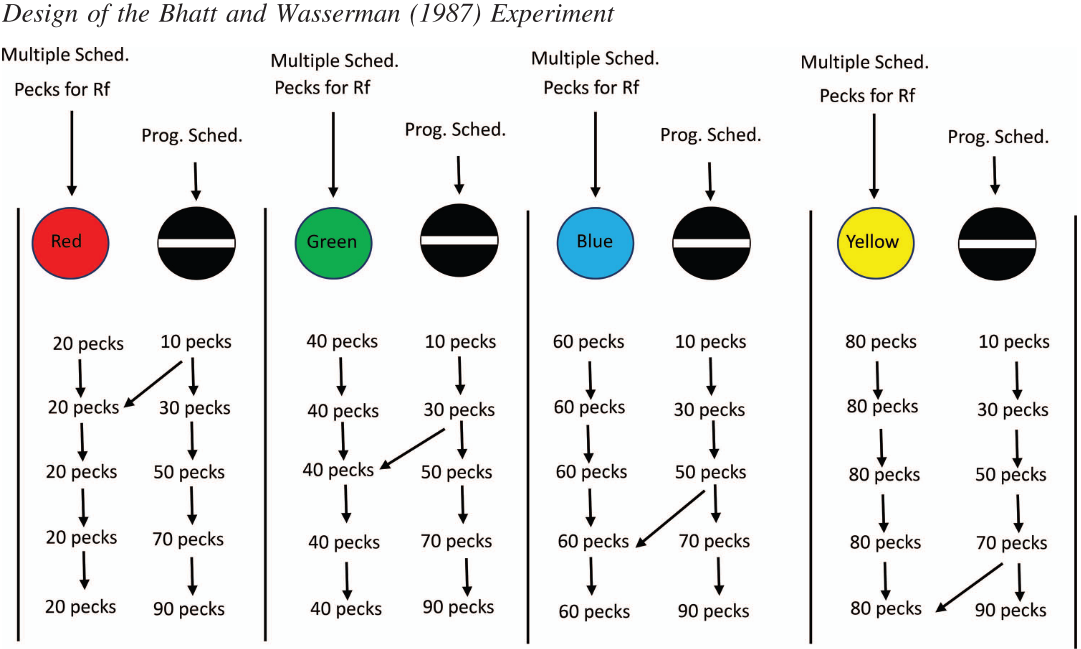
\includegraphics[scale=0.5]{Chandel2021(1).png}
		\caption{Puntos óptimos para cambiar de un programa de razón progresiva a uno fijo.}
	\end{center}
\end{figure}

Es posible que los resultados se deban a que la evolución seleccionó factores de sesgo no incluidos en el procedimiento, como el desconocimiento de la riqueza de parches alternativos, del tiempo de viaje, o de los riesgos asociados. Sin embargo, estos factores hubiesen hecho a los animales permanecer {\itshape más} de lo que sería óptimo.

Una explicación alternativa es patrón serial general de los reforzadores. Hay evidencia que indica que los animales son sensibles a los decrementos sistemáticos en los programas de reforzamiento.

En un programa progresivo el incremento sistemático de la razón y la cantidad de respuestas requeridas para el reforzador recién obtenido indican al animal que la situación está empeorando. Se podría decir que los animales son influidos no solo por el requisito del siguiente reforzador, sino también por el de reforzadores aun más adelantados.

Otro hallazgo de ese procedimiento fue una relación no-monotónica entre la alternativa con el programa fijo y el grado en que las palomas abandonaban prematuramente la alternativa progresiva. Cuando se requerían pocas respuestas en el programa fijo, las palomas eran cercanas al óptimo. Cuando se requería una cantidad media, abandonaban temprano. Cuando se requería una cantidad grande, de nuevo estaban cerca de lo óptimo. Una posible razón sería que la diferencia entre el programa progresivo más corto (10) y el fijo más corto (20) era igual a la diferencia entre los dos programas más largos (70 y 80). Quizá si la disparidad entre los números de respuestas requeridas para el reforzamiento hubiese sido proporcional al número absoluto de respuestas, los resultados hubiesen sido diferentes.

Además, en el procedimiento cambiar a la alternativa fija temprano demora un poco más el primer reforzador, pero hace que todos los posteriores vengan más pronto que si no hubiesen cambiado.

Para controlar esa posibilidad en este experimento cambiar al programa fijo le daba a las palomas solo un reforzador por ensayo y le ponía fin. Así, abandonar temprano el programa progresivo resultaba en más respuestas hasta el siguiente reforzador y en menos reforzadores totales.

El propósito del experimento es determinar si la conducta de las palomas es capturada por una forma simple de la teoría de forrajeo óptimo o por una forma de aprendizaje serial de patrones.

{\scshape\bfseries Method}

Se utilizaron 8 palomas en una caja operante con 3 teclas. 

Las palomas fueron pre-entrenadas para picar la tecla izquierda para recibir comida. 6 veces cuando era roja, 11 veces cuando verde, 23 cuando azul, y 45 cuando amarilla. Entremezclados en esos ensayos había ensayos a la tecla derecha iluminada con tres líneas verticales con un requisito de respuesta que cambiaba aleatoriamente entre valores de 4, 8, 16, 32, o 64.

En el procedimiento cada ensayo comenzó con la presentación simultánea de la razón progresiva señalada por la tecla con barras verticales, que sucesivamente requería 4, 8, 16, 32 y 64 respuestas, y uno de los cuatro colores de la tecla complementaria. Cada colo señalaba un requisito de respuesta. Los requisitos de la alternativa fija eran la media de los dos requisitos de la alternativa progresiva que la rodeaban. Las palomas podía picar en ambas teclas, pero una vez cumplido el requisito en la alternativa fija u obtenido el quinto reforzador, se acababa el ensayo. La estructura de la tarea se presenta en la figura 2.

\begin{figure}[ht]
	\begin{center}
		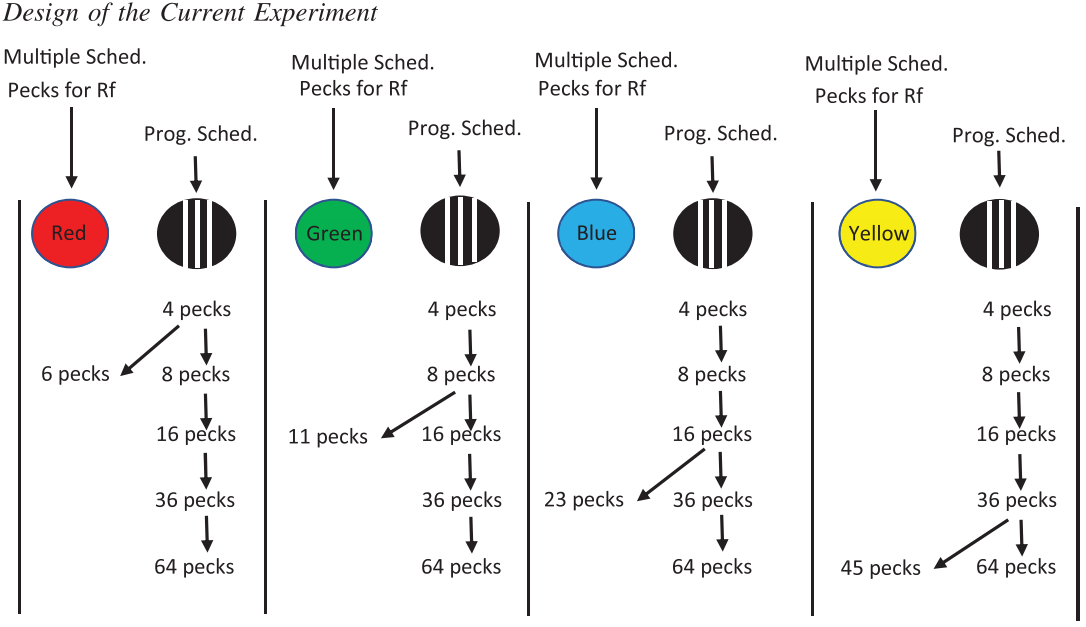
\includegraphics[scale=0.5]{Chandel2021(2).png}
		\caption{Estructura de la tarea.}
	\end{center}
\end{figure}

Los ensayos estaban separados por un intervalo entre ensayos de 10 segundos. Cada sesión tenía 24 ensayos, 6 con cada color, presentados al azar. Se corrieron 40 sesiones.

{\bfseries Forced trials}

Dos palomas se sesgaron a una tecla. Para ellas, la mitad de los 24 ensayos eran forzados con una sola tecla (la menos preferida). Los demás ensayos eran de elección.

{\bfseries Analyses}

Se usó la media del número de reforzadores obtenidos en el programa progresivo de las últimas 10 sesiones para cada estímulo. Ese número fue comparado con el número óptimo para cada color: uno para rojo, dos para verde, tres para azul, y cuatro para amarillo.

Las palomas abandonaron el programa progresivo significativamente más temprano de lo que sería esperado si abandonaran en puntos óptimos. La diferencia entre lo observado y lo óptimo es pequeña en rojo, crece hacia verde y azul, y se vuelve prácticamente nula en amarillo: la misma tendencia observada en experimentos anteriores. Las palomas abandonaron antes de lo óptimo en todos los colores salvo en amarillo, que señalaba los programas con razón más alta.

El análisis se repitió usando la proporción relativa entre observado y óptimo y se encontró de nuevo que las palomas abandonaban más temprano de lo que sería óptimo.

{\scshape\bfseries Discussion}

Se confirma el hallazgo de Bhatt y Wasserman que indica que las palomas abandonan antes de lo predicho por la teoría de forrajeo óptimo.

La teoría de forrajeo óptimo predice que deberían permanecer más tiempo en el programa progresivo debido a (1) sesgos inherentes en la incertidumbre de la naturaleza, o (2) porque aun al cambiar al programa fijo para minimizar el tiempo y número de respuestas al siguiente reforzador, las palomas estarían abandonando reforzadores adicionales que serían obtenidos en el programa progresivo. Aunque es difícil hacer predicciones con la teoría de forrajeo óptimo debido a que los animales son influidos por otros factores como los tiempos variables de viaje entre parches, historia previa de reforzamiento, y peligros potenciales. Aunque esos factores alentarían al organismo a esperar {\itshape más} y no {\itshape menos}.

Abandonar temprano también viola el principio conductual del menor esfuerzo debido a que deben realizar más respuestas de las que hubieran hecho de haber permanecido. También se viola la hipótesis de reducción de la demora debido a que al permanecer en el programa progresivo más tiempo, la demora al siguiente reforzador hubiese sido menor.

Esta tendencia a abandonar antes de lo óptimo es similar a la {\itshape precrastinación}, la tendencia a iniciar o completar tareas antes de lo necesario, incluso cuando hacerlo es más costoso.

En humanos esta tendencia se ha atribuido a un deseo por completar las sub-metas pronto evitando olvidarlas después. Aunque parece requerirse de cierto pensamiento que haría que el fenómeno no exista en otros animales, el hecho es que se encontró aquí.

Una explicación está en la tendencia de los animales a preferir programas señalados (múltiples) sobre no señalados (mixtos). El programa progresivo no era señalado, aunque usualmente este tipo de programas no ofrecen forma de predecir la siguiente entrega y el programa de este experimento sí lo hacía.

Aunque se maximizaría el número de reforzadores por ensayo al permanecer hasta el final, las palomas abandonaban temprano. Quizá a ello contribuyó la saliencia de las teclas de colores.

También es posible que las palomas hayan sido sensibles al {\itshape patrón serial} y supieran que el programa se iba adelgazando. El patrón serial puede haber potenciado el valor negativo del efecto del número de respuestas requerido para el siguiente reforzador. Esta explicación podría decir por qué las palomas estuvieron cerca de la optimalidad en el programa fijo del mayor requisito de respuesta: en esos ensayos la opción óptima sería permanecer hasta las 32 respuestas requeridas en el programa progresivo. Después de eso, el programa progresivo requiere de 64 respuestas mientras que el fijo solo 45. El paso de 32 a 64 podría no ser un factor suficiente para sobreponerse al número adicional de respuestas para cambiar al programa fijo.

Estos resultados sumados a los de Bhatt y Wasserman indican que los animales son sensibles a los patrones estructurales de las secuencias de eventos, y que incluso eventos simples como la ocurrencia de reforzadores en patrones pueden disparar procesos cognitivos complejos.


\end{document}
